\begin{ZhChapter}

\chapter{Purposed Algorithm}
This section will provide a brief overview of the contents that will be discussed in this chapter: Section 3.1 will introduce the architecture of our algorithm and use a simple flowchart to provide a basic introduction to the proposed algorithm. Section 3.2 will provide a detailed description of our software and hardware specifications, as well as the setup procedures. Section 3.3 will provide an in-depth explanation of our proposed algorithm, including the underlying concepts and the rationale behind our approach.
\section{The Architecture of Algorithm}

\section{Experimental Environment Setup}

\section{Main Method}
% \subsection{}
% 定義定義定義定義定義定義\cite{latex2e},定義定義定義定義,定義定義定義定義定義定義定義定義定義定義,定義定義。

% \begin{table*}[htbp]
%     \centering
%     \caption{表格範例標題} \label{tab: complexity}
%     \makebox[\linewidth][c]{
%     \renewcommand\arraystretch{1.2}{
%         \begin{tabular}{| l | c  c  c  c |}
%         \hline
%         Protocol & $P$ & $CS_1$ & $CS_2$ & $RG$ \\
%         \hline
%         MSSMul & $O(1)$, $O(1)$, N/A & $O(n-t)$, $O(n)$, $O(1)$ & $O(n-t)$, $O(n)$, N/A & $O(1)$, $O(n)$, $O(n)$ \\
%         SC & $O(1)$, $O(1)$, N/A & $O(n-t)$, $O(n)$, $O(1)$ & $O(n-t)$, $O(n)$, N/A & $O(1)$, $O(n)$, $O(n)$ \\
%         \hline 
%         \end {tabular}
%     }}
% \end {table*}

% \section{模型說明(小標)}

% 說明說明說明說明,說明說明說明說明說明說明說明說明說明說明說明說明,說明說明說明說明說明說明說明說明。

% \begin{figure*}[htbp]
%     \centering
%     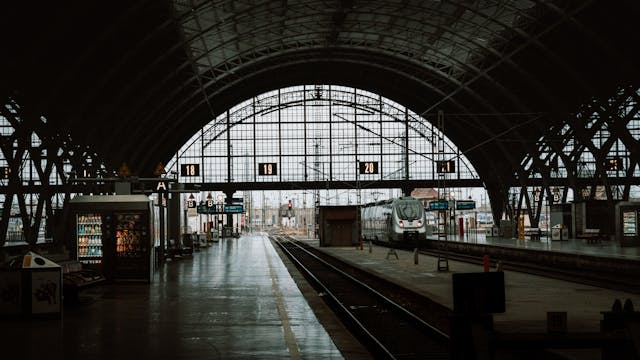
\includegraphics[width = 0.5\textwidth]{image.jpeg}
%     \caption{Cool train station}
%     \label{fig: image}
% \end{figure*}

\end{ZhChapter}